\documentclass{article}
\usepackage{amssymb,amsmath}
\usepackage[mathletters]{ucs}
\usepackage[utf8x]{inputenc}
% Redefine labelwidth for lists; otherwise, the enumerate package will cause
% markers to extend beyond the left margin.
\makeatletter\AtBeginDocument{%
  \renewcommand{\@listi}
    {\setlength{\labelwidth}{4em}}
}\makeatother
\usepackage{enumerate}
\usepackage{array}
% This is needed because raggedright in table elements redefines \\:
\newcommand{\PreserveBackslash}[1]{\let\temp=\\#1\let\\=\temp}
\let\PBS=\PreserveBackslash
\usepackage{url}
\usepackage{graphicx}
% We will generate all images so they have a width \maxwidth. This means
% that they will get their normal width if they fit onto the page, but
% are scaled down if they would overflow the margins.
\makeatletter
\def\maxwidth{\ifdim\Gin@nat@width>\linewidth\linewidth
\else\Gin@nat@width\fi}
\makeatother
\let\Oldincludegraphics\includegraphics
\renewcommand{\includegraphics}[1]{\Oldincludegraphics[width=\maxwidth]{#1}}
\usepackage[breaklinks=true,unicode=true,pdfborder={0 0 0}]{hyperref}
\setlength{\parindent}{0pt}
\setlength{\parskip}{6pt plus 2pt minus 1pt}
\usepackage{listings}
\usepackage[top=2cm,bottom=2cm,left=2cm,right=2cm,a4paper]{geometry}
\usepackage[frenchb]{babel}
\usepackage{graphicx}
\usepackage{color}
\definecolor{vert}{rgb}{0,0.5,0}
\definecolor{bleu}{rgb}{0,0,0.5}
\lstset{basicstyle=\ttfamily\small}

\title{Formation scribe}
\author{Nicolas Poulain - Dafor 2012}

\begin{document}
\maketitle

\tableofcontents

\section{Les modules EOLE}

Extrait de \url{http://eole.orion.education.fr/index.php/home}

\begin{figure}[htbp]
\centering

\includegraphics{scribe_html_2ce1ff75.png}
\caption{Logo EOLE}
\end{figure}

Eole est un projet collaboratif basée sur la philosophie du logiciel
libre. La mutualisation des compétences et des moyens permet de réaliser
des solutions économiques, fiables et performantes.

Chaque module constitue une distribution GNU/LINUX spécifique qui permet
d'installer facilement un serveur dédié. Les services offerts sont
pré-configurés, l'ensemble est cohérent. Vous devez télécharger sur ce
site l'image ISO qui vous permettra de graver un DVD ou un CD
d'installation. Ce DVD/CD est multi module, le choix du module à
installer est proposé au démarage (boot).

Les modules sont disponibles en deux versions

\begin{center}
\begin{tabular}{ll}
EoleNg 2.2 & EoleNg 2.3\\
\hline
- Disponible depuis le 16 Janvier 2009. & - Disponible depuis le 8 Juin
2011.\\
- basée sur la version 8.04 Ubuntu & - basée sur la version 10.04
Ubuntu\\
- Arrêt du support mises à jour : Juin 2013 & - Arrêt du support mises à
jour : Juin 2015\\
\end{tabular}
\end{center}

\subsection{Scribe : Un serveur pédagogique complet.}

Scribe est un contrôleur de domaine dotée de fonctions évoluées. Il
optimise la gestion de votre parc de stations clientes. Il dispose d'un
annuaire qui référence, élèves, parents, personnels enseignant et
administratifs, il propose un service de messagerie et héberge vos
applications web au sein d'un portail Web 2.0.

Scribe est un contrôleur de domaine. - gestion des connexions réseau des
utilisateurs ; - partage de fichiers et de répertoires ; - support des
ACL ; - partage d'imprimantes ; - gestion des comptes utilisateurs et
des accès ; - exécution d'applications utilisateurs ;

Scribe est un système de messagerie articulé autour d'un annuaire
performant. - l'annuaire est initialisé à partir d'importation de
comptes (SCONET, BE1D, AAF, CSV,\ldots{}) ; - l'annuaire peut servir de
base d'authentification pour d'autres services réseaux ; - la messagerie
gère deux domaines distincts (l'Internet et l'intranet académique) ; -
utilisation au choix d'une interface web multilingue ou d'un client de
messagerie standards. - un service de listes de diffusion ; - une
sécurité anti­spam, un anti­virus, une gestion de quotas (taille des
boites aux lettres)

Scribe offre des services web - un serveur web; - un portail web; - des
applications pré-installés

Scribe est un serveur d'authenfication unqiue (SSO) - Eole SSO Utilise
l'annuaire LDAP - Les standards C.A.S 2 et OpenID sont supportés - La
féération d'identité est possible via le protocole SAML.

Scribe dispose d'une gestion avancée des utilisateurs et des postes
clients - Distribution de devoir - Controle d'acces à Internet et au
services réseaux - appliquer des restrictions ou pré­configurer des
applications, en fonction du login de l'utilisateur ou de ses groupes et
du nom de la machine sur laquelle il se connecte ; - effectuer des
actions distantes sur les stations (fermer la session, éteindre ou
redémarrer un ou plusieurs postes) ; - surveiller la détection de virus
par le serveur ;

\subsection{Schéma d'un réseau d'établissement}

Sur l'académie de Paris, les réseaux d'établissement sont organisés par
la DSI, service informatique du Rectorat qui assure en plus
l'administration et la maintenance des serveurs Amon, Scribe et Horus.
Voir figure \ref{2149feac}.

\begin{figure}[htbp]
\centering
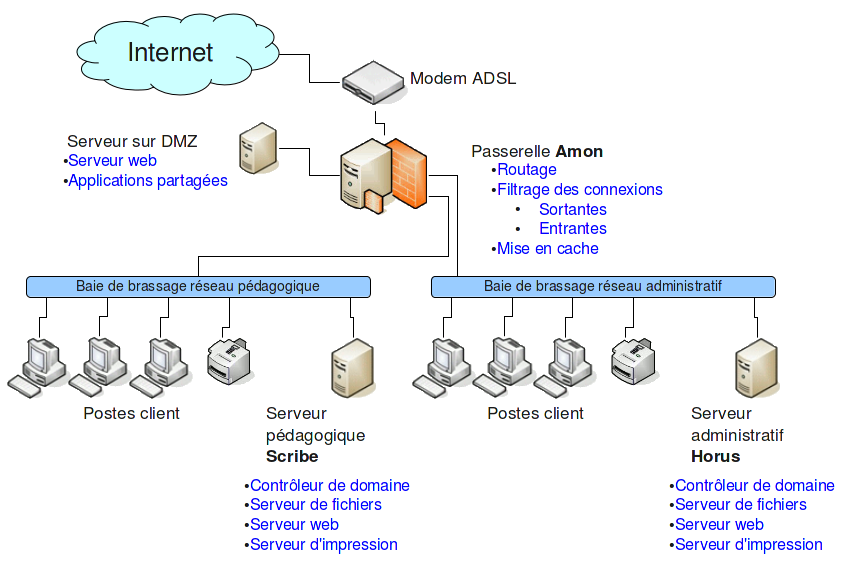
\includegraphics{scribe_html_2149feac.png}
\caption{\label{2149feac}}
\end{figure}

Les établissements assurent par eux-même les tâches de gestion courante
du réseau et des machines avec les droits qui leur sont laissé en
utilisant au travers des interfcaes de gestion de ces serveurs.

\subsection{Déroulement de la formation}

Durant cette formation, nous allons simuler un réseau d'établissement
grâce à des machines virtuelles. Cela nous permettra de contrôle
complètement tous les éléments, d'effectuer tous les tests sans risque
pour les machines réelles et le réseau qui nous entourent.

Sur la figure suivante, on simule plusieurs machines sur une seule
appelée machine hôte. Un poste windows virtuel est un ordinateur virtuel
sur leque a été installé un système d'exploitation comme on le fait sur
une machine réelle.

\begin{figure}[htbp]
\centering
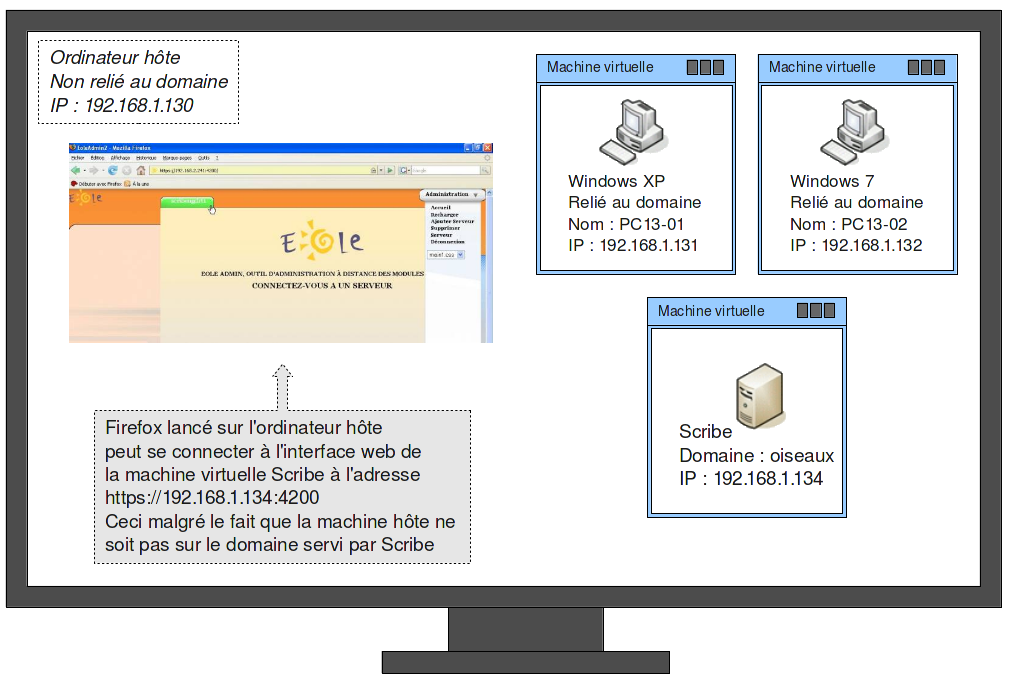
\includegraphics{scribe_html_413f4ff1.png}
\caption{\label{413f4ff1}}
\end{figure}

La situation décrite sur la figure \ref{413f4ff1} est équivalente à
celle de la figure \ref{78733841}.

\begin{figure}[htbp]
\centering
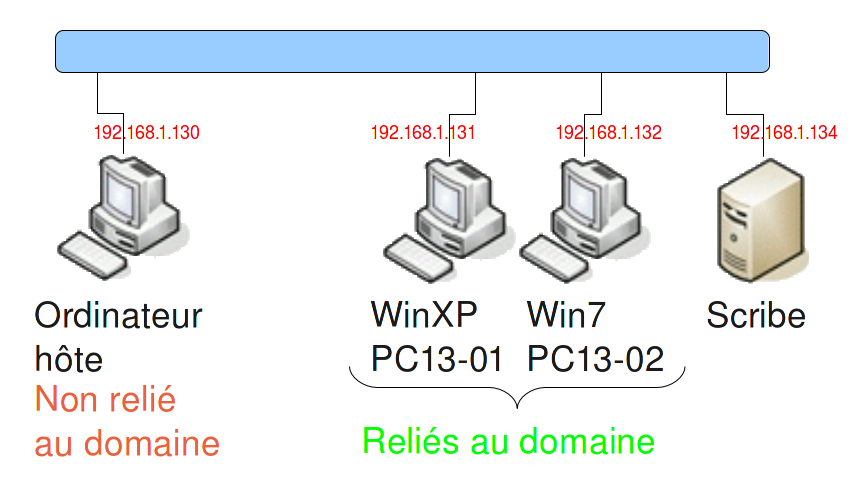
\includegraphics{scribe_html_78733841.png}
\caption{\label{78733841}}
\end{figure}

Notre travail maintenant est de créer la machine virtuelle qui va
accueillir le sytème d'exploitation Linux sur lequel fonctionne.

Après avoir demandé la création d'une nouvelle machine dans VirtualBox,
puis donné un nom (disons scribe) et choisi le type de système
d'exploitaion (ici Linux-Ubuntu), passez toutes les étapes en acceptant
les choix par défaut (sauf pour la mémoire vive que nous passerons de
512Mo à 256Mo).

Une fois ces opérations terminées, - cocher la case «Activer PAE/NX»
dans l'onglet «Processeur» de la section «Système» de votre machine
virtuelle. - choisir le mode d'accès par pont pour la carte réseau 1.
Elle prendra ainsi une adresse sur le réseau sur lequel se trouve la
machine hôte. - L'image iso du dvd eole, téléchargée sur le site Eole
\url{http://eoleng.ac-dijon.fr/pub/iso/} doit être monté comme un cd(ou
dvd) virtuel, pour cela cliquez sur l'icône cd-rom dans l'onglet
«Stockage», comme sur l'image ci-dessous puis naviguez dans
l'arborescence pour indiquer le fichier .iso.

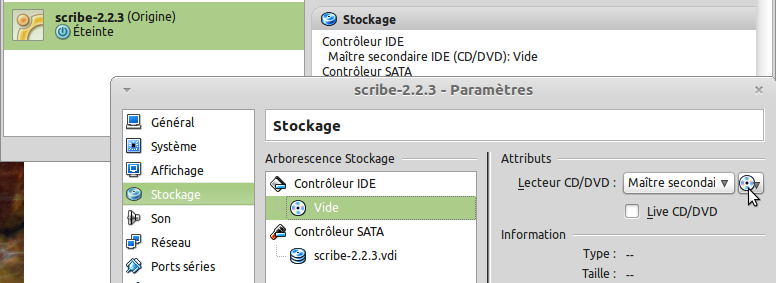
\includegraphics{scribe_html_m69a9bc5b.png}\\ On peut alors mettre en
marche la machine virtuelle.

\section{Mise en place du serveur}

\subsection{Installation}

\begin{figure}[htbp]
\centering
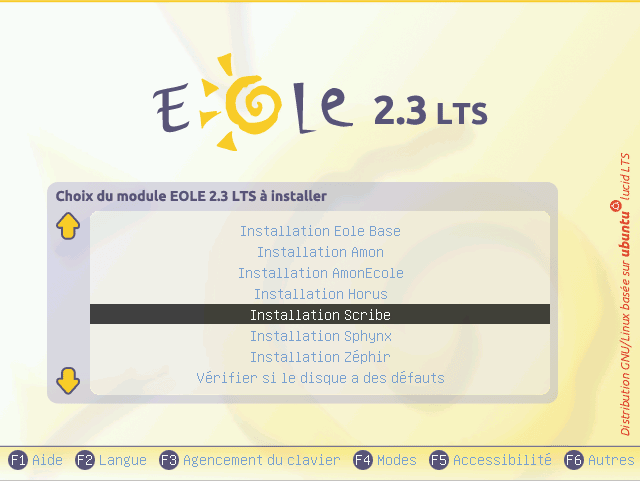
\includegraphics{scribe_html_m1451a7db.png}
\caption{image}
\end{figure}

Après avoir vérifié au niveau du BIOS que la machine démarre
prioritairement sur le CD, le menu ci-contre apparaît.

Une bonne idée consiste à vérifier si le disque (le CD) a des défauts
afin d'éviter de perdre du temps avec une installation qui échouerait
sans doute.

Une fois ceci fait, lançons l'installation de Scribe. La procédure est
automatique et vous n'avez qu'à observer les étapes

\begin{figure}[htbp]
\centering
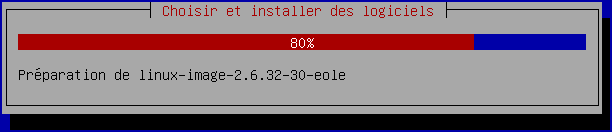
\includegraphics{scribe_html_4b5e166b.png}
\caption{image}
\end{figure}

Après redémarrage, le gestionnaire de démarrage GRUB vous propose
plusiers entrées. Nous choisissons celle par défaut

\begin{figure}[htbp]
\centering
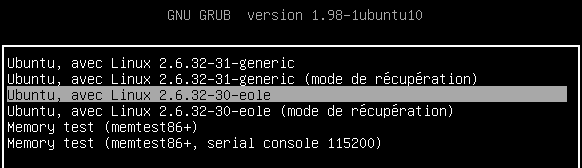
\includegraphics{scribe_html_m6522c87a.png}
\caption{image}
\end{figure}

Vous pouvez maintenant vous identifier avec le login «root».

\begin{itemize}
\item
  Pour scribe 2.2, le mot de passe est \lstinline!eole!,
\item
  Pour scribe 2.3, le mot de passe est \lstinline!$eole&123456$!.
\end{itemize}
Avant de nous lancer dans la configuration de notre contôleur de domaine
scribe, notons ici quelques informations réseau dont nous aurons besoin
pour configurer notre serveur :

\begin{itemize}
\item
  L'adresse IP fixe que nous allons lui attribuer : \_ \_ \_ . \_ \_ \_
  . \_ \_ \_ . \_ \_ \_
\item
  Le masque de sous-réseau : \_ \_ \_ . \_ \_ \_ . \_ \_ \_ . \_ \_ \_
\item
  L'adresse de broadcast : \_ \_ \_ . \_ \_ \_ . \_ \_ \_ . \_ \_ \_
\item
  L'adresse IP du ou des serveur(s) DNS :
  \begin{itemize}
  \item
    \_ \_ \_ . \_ \_ \_ . \_ \_ \_ . \_ \_ \_
  \item
    \_ \_ \_ . \_ \_ \_ . \_ \_ \_ . \_ \_ \_
  \end{itemize}
\item
  Le nom que nous donnerons à la machine :
\item
  Le nom du domaine auquel les clients vont s'authentifier :
\item
  Le mot de passe root\footnote{root : utiisateur linux ; a tous les
    droits sur le serveur

    scribe : utilisateur linux ; peut faire certains tests via une
    interface graphique

    admin : utilisateur samba ; gestionnaire des machines une fois
    celles-ci connectées au domaine , c'est l'administrateur réseau).} :
  \lstinline"dog!cat$mouse"
\item
  Le mot de passe eole ou scribe : \lstinline"fox!bird$fly"
\item
  Le mot de passe admin : \lstinline!plop!
\end{itemize}
Mise à jour :

\lstinline!root@scribeng:~# Maj-Auto -i!

Saisissez la commande \lstinline!gen_config! qui va lancer le générateur
de configuration

\lstinline!root@scribeng:~# gen_config!

La série d'écrans est à renseigner en étant très attentif.

\subsubsection{Configuration scribe 2.2}

Voir fugures \ref{m4d52829f} à \ref{m44b07c21}.

\begin{figure}[htbp]
\centering
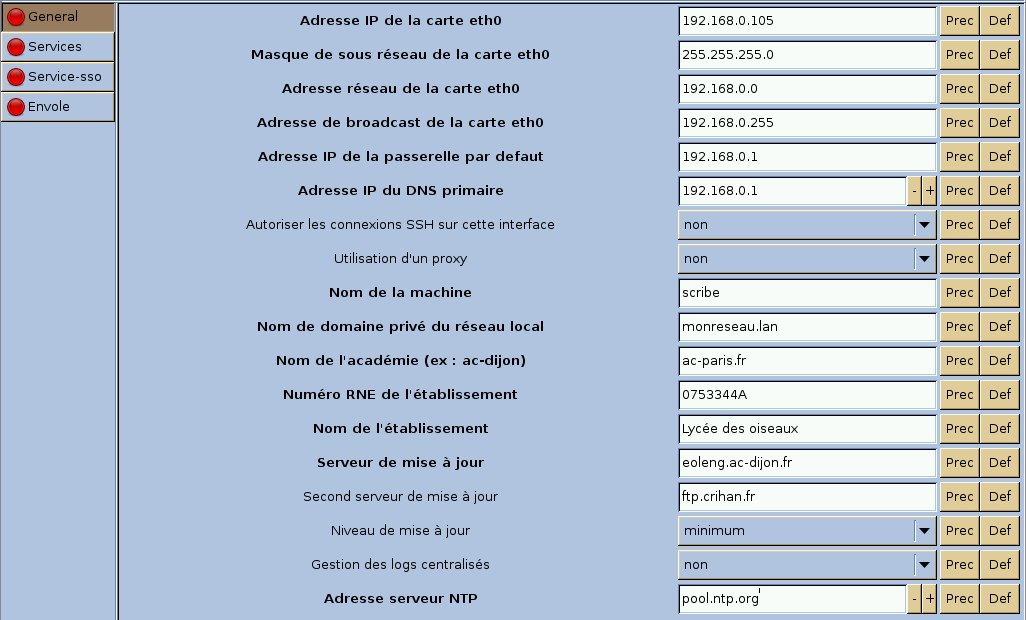
\includegraphics{scribe_html_m4d52829f.jpg}
\caption{Scribe 2.2 \label{m4d52829f}}
\end{figure}

\begin{figure}[htbp]
\centering
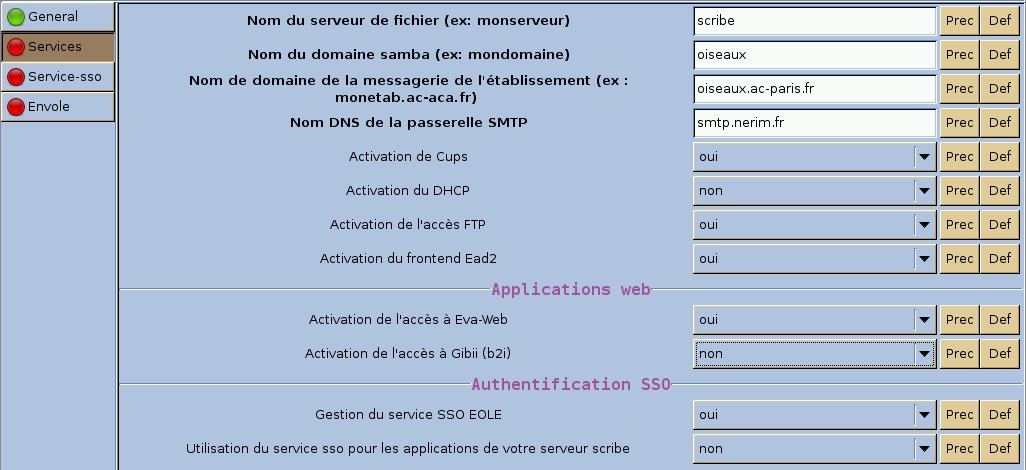
\includegraphics{scribe_html_1f004f88.jpg}
\caption{Scribe 2.2}
\end{figure}

\begin{figure}[htbp]
\centering
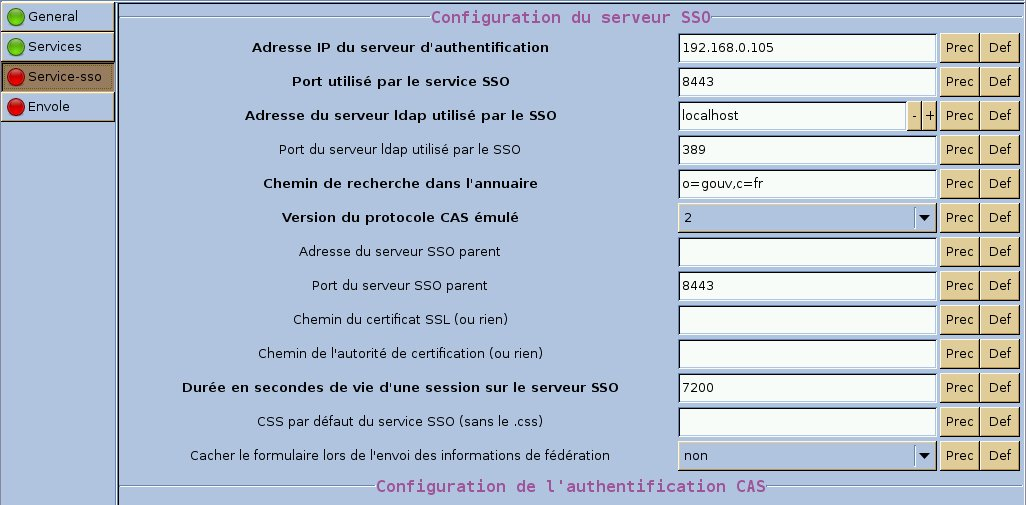
\includegraphics{scribe_html_m5ada8c94.jpg}
\caption{Scribe 2.2}
\end{figure}

\begin{figure}[htbp]
\centering
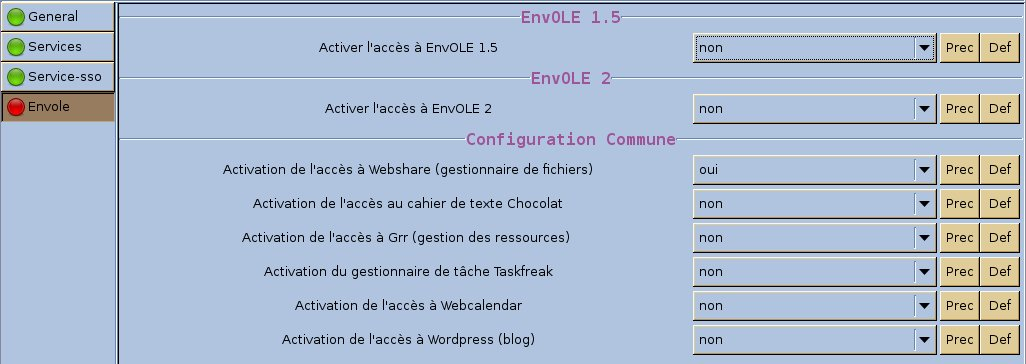
\includegraphics{scribe_html_m44b07c21.jpg}
\caption{Scribe 2.2 \label{m44b07c21}}
\end{figure}

\subsubsection{Configuration scribe 2.3}

Voir fugures \ref{5dc039bc} à \ref{m6ec096b1}.

\begin{figure}[htbp]
\centering
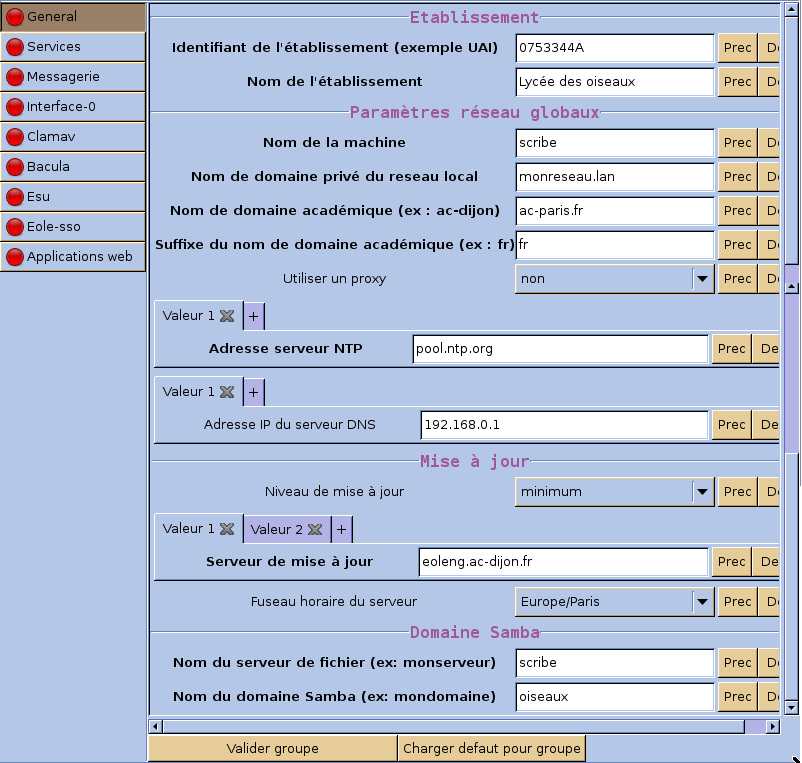
\includegraphics{scribe_html_5dc039bc.png}
\caption{Scribe 2.3 \label{5dc039bc}}
\end{figure}

\begin{figure}[htbp]
\centering
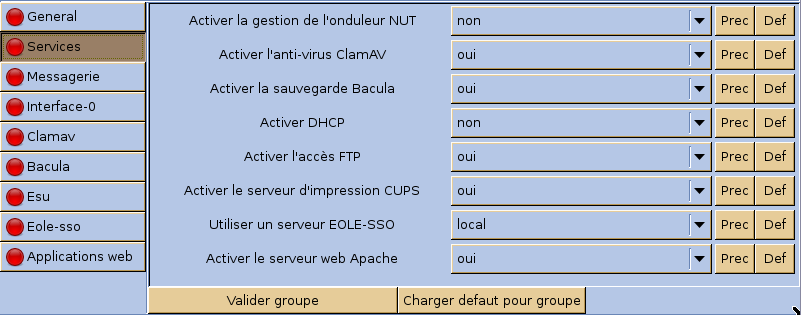
\includegraphics{scribe_html_m291b378c.png}
\caption{Scribe 2.3}
\end{figure}

\begin{figure}[htbp]
\centering
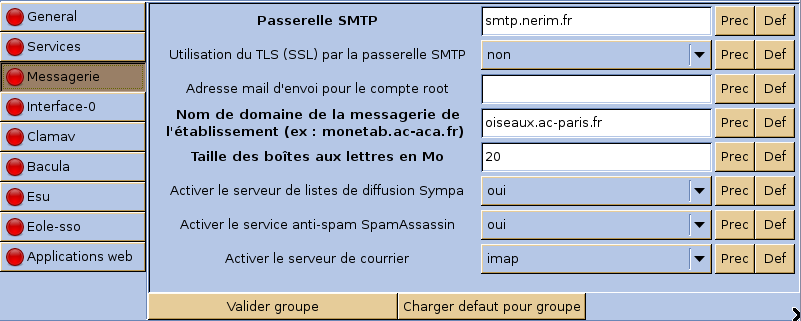
\includegraphics{scribe_html_m408bb4bb.png}
\caption{Scribe 2.3}
\end{figure}

\begin{figure}[htbp]
\centering
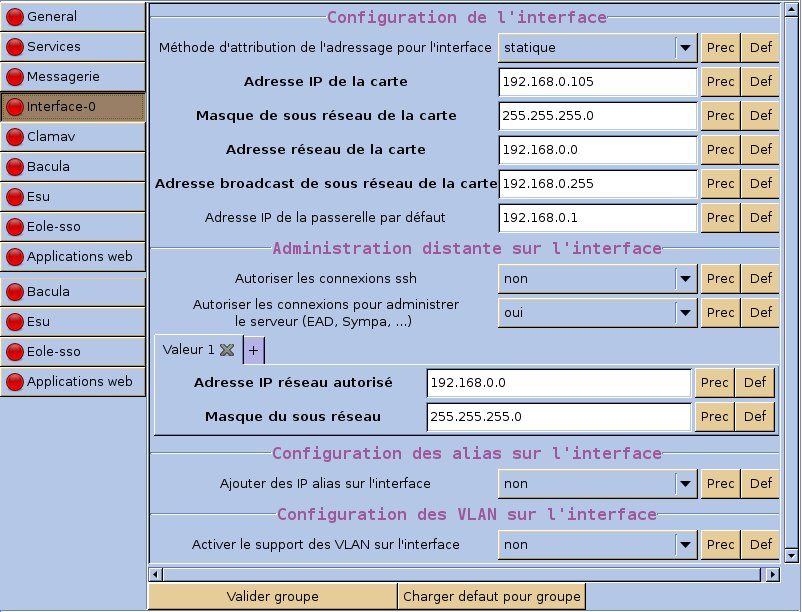
\includegraphics{scribe_html_43381116.jpg}
\caption{Scribe 2.3}
\end{figure}

\begin{figure}[htbp]
\centering
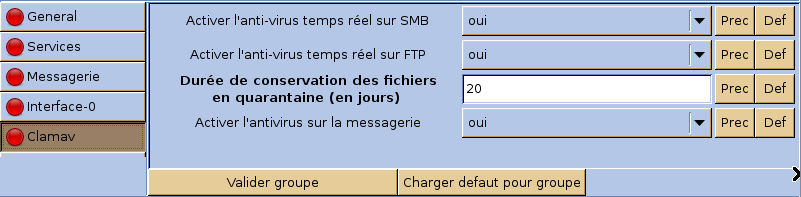
\includegraphics{scribe_html_m672d0ca.png}
\caption{Scribe 2.3}
\end{figure}

\begin{figure}[htbp]
\centering
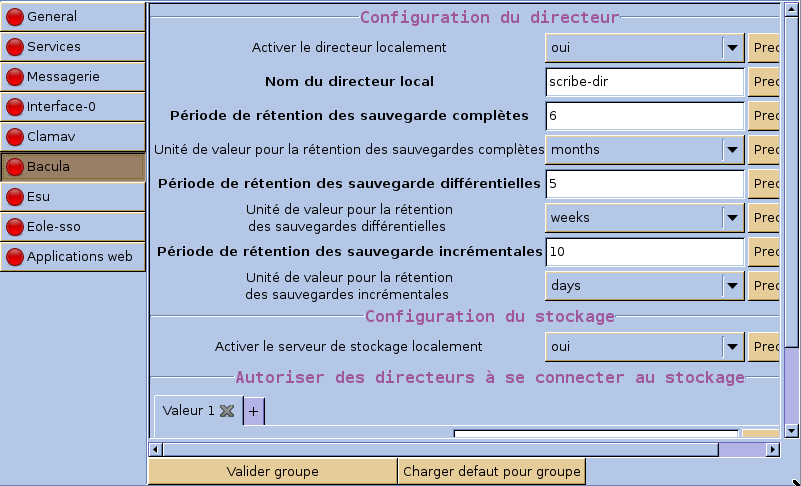
\includegraphics{scribe_html_71d87af7.png}
\caption{Scribe 2.3}
\end{figure}

\begin{figure}[htbp]
\centering
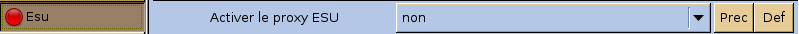
\includegraphics{scribe_html_m51dc1543.png}
\caption{Scribe 2.3}
\end{figure}

\begin{figure}[htbp]
\centering
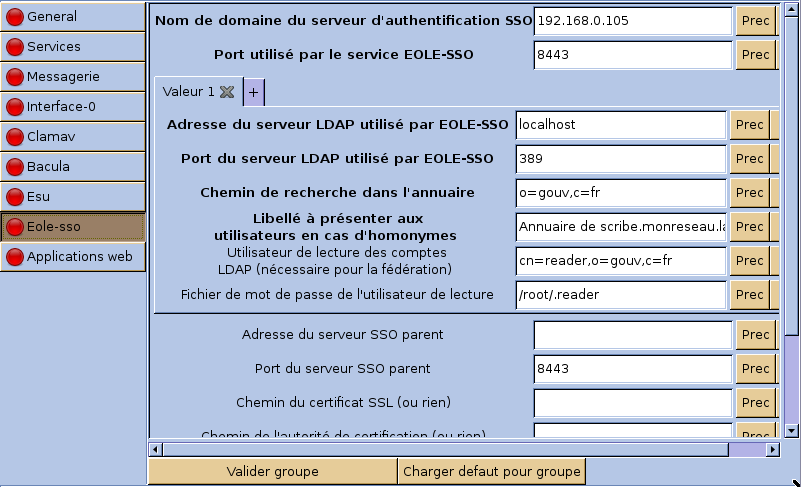
\includegraphics{scribe_html_28489be3.png}
\caption{Scribe 2.3}
\end{figure}

\begin{figure}[htbp]
\centering
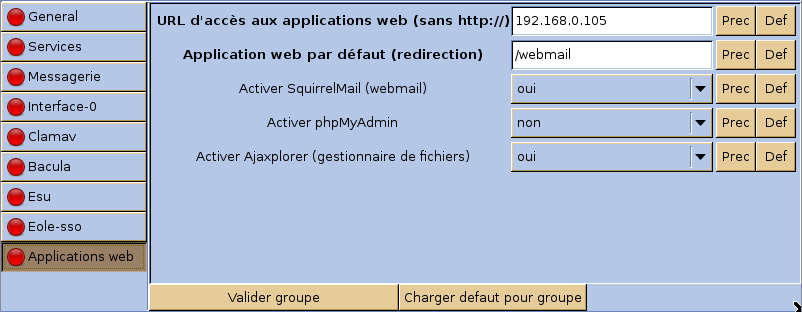
\includegraphics{scribe_html_m6ec096b1.png}
\caption{Scribe 2.3 \label{m6ec096b1}}
\end{figure}

\subsubsection{Instanciation}

Après avoir rempli les champs, on peut enregistrer ces paramètres qui
vont constituer un fichier nommé «zephir.eol» dont le rôle est de donner
les instructions au programme d'instanciation instance.

\lstinline!root@scribeng:~# instance zephir.eol!

Au cours de l'exécution du programme, il vous sera demandé de changer
les mots de passe

\begin{itemize}
\item
  du super administrateur Linux nommé «root»;
\item
  de l'administrateur scribe restreint nommé «eole» ou «scribe»
\item
  de l'admistrateur du domaine nommé «admin».
\end{itemize}
Lors de l'installation, le programme vous proposera sans doute des
télécharger des mises à jour il est essentiel d'accepter car elles
corrigent des problèmes de sécurité comme elles apportent des
améliorations des programmes de la distribution Ubuntu mais aussi de la
suite Scribe développée par l'académie de Dijon.

À la fin du processus, après construction des bases de données et
exécution de tous les scripts de pré/postinstance, la machine doit
redémarrer.

\subsubsection{Pourquoi n'utiliser instance qu'une seule fois ?}

Un fois les modifications apportées au fichier config.eol, on se gardera
bien de relancer le programme d'instanciation instance. En effet il
poserait des questions inutiles, pourrait effacer des comptes, perturber
gravement les connexions au domaine des machines déjà intégrées.

En cas de changement sur le réseau ou d'erreur lors de la configuration,
il est possible de relancer la commande gen\_config afin de modifier le
fichier /etc/eole/config.eol. Pour ensuite lancer une reconfiguration
avec le programme reconfigure. dont la fonction est de lire le fichier
/etc/eole/config.eol pour en appliquer les paramètres aux différents
services en fonctionnement.

\begin{lstlisting}
root@scribeng:~# gen_config /etc/eole/config.eole
root@scribeng:~# reconfigure
\end{lstlisting}
\subsection{Intégration des clients au domaine}

\begin{itemize}
\item
  Première étape : faire entrer les machines windows dans le domaine. La
  copie d'écran suivante montre l'utilisateur admin faisant entrer dans
  le domaine une machine sous WindowsXP

  \begin{figure}[htbp]
  \centering
  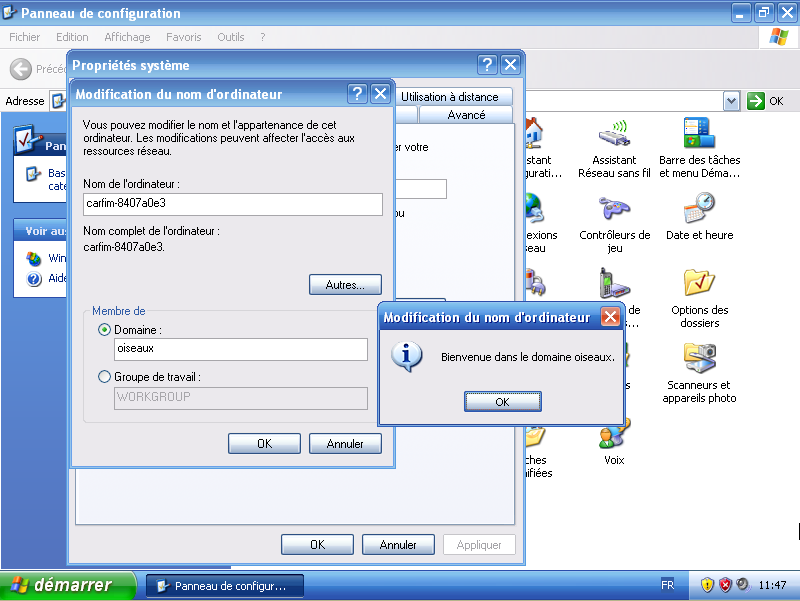
\includegraphics{scribe_html_78aacfe6.png}
  \caption{intégration au domaine}
  \end{figure}
\item
  Deuxième étape : installer le client scribe.

  Après redémarrage et connexion en tant qu'admin sur le domaine,
  rendons-nous dans le poste de travail puis dans le répertoire
  personnel nommé U: Nous allons exécuter le programme
  \lstinline!Install_Client_Scribe!.

  \begin{figure}[htbp]
  \centering
  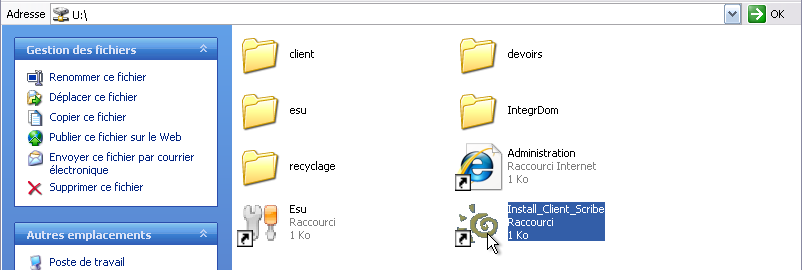
\includegraphics{scribe_html_m4358be12.png}
  \caption{Installation du client scribe}
  \end{figure}
\end{itemize}
\section{L'E.A.D. (Eole ADmininistration)}

\subsection{Présentation}

L'EAD est une interface WEB qui permet de faire l'administration de
premier niveau de toutes les composantes du serveur Scribe : système,
messagerie, utilisateurs, groupes,\ldots{} Il offre également aux
professeurs la possibilité de modifier leurs préférences, gérer les
élèves, les groupes dont ils sont responsables\ldots{}

L'accès à l'EAD se fait depuis le navigateur web FIREFOX ou CHROME (mais
PAS Internet Explorer) avec l'URL suivante :
\url{https://srv-scribe:4200/} (ou \url{https://xxx.xxx.xxx.xxx:4200}
avec l'adresse IP du serveur Scribe).

\begin{figure}[htbp]
\centering
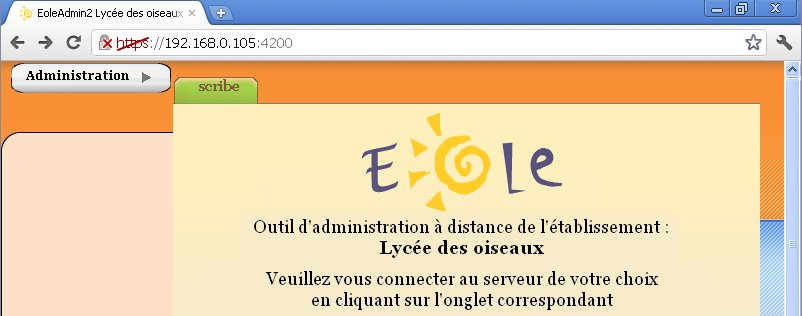
\includegraphics{scribe_html_661f3efb.jpg}
\caption{L'EAD}
\end{figure}

Cliquez sur scribe puis à la connexion entrez le nom d'utilisateur et le
mot de passe associé.

En tant qu'administrateur, vous allons créer la base des élèves de
l'établissement à partir des fichiers zip ou xml récupérés depuis sconet
(fichiers exemple sur \url{http://cjoint.com/?0AiqKCRRtW3}):

\begin{itemize}
\item
  \lstinline!ExportXML_ElevesSansAdresses.zip! ou
  \lstinline!ElevesSansAdresses.xml!
\item
  \lstinline!ExportXML_Nomenclature.zip! ou \lstinline!Nomenclature.xml!
\item
  \lstinline!ExportXML_Structures.zip! ou \lstinline!Structures.xml!
\end{itemize}
Dans l'EAD, cliquez Outils puis successivement sur Importation
-\textgreater{} Importation annuelle des bases. Choisissez ensuite
«Sconet» puis «Élèves seulement». Les trois fichiers seront traités pour
intégrer les élèves au système en créant leurs identifiants et mots de
passe selon vos préférences.

Les profils utilisateurs représentent l'environnement par défaut des
utilisateurs. Il existe trois types de profils :

\begin{itemize}
\item
  le profil local : il est stocké sur la station Windows,
  l'environnement est donc modifié lorsque l'utilisateur change de poste
\item
  le profil itinérant : il est stocké dans le répertoire personnel de
  l'utilisateur, l'environnement suit l'utilisateur
\item
  les profils obligatoires : ils sont stockés dans un répertoire commun,
  l'environnement est le même pour tous mais il faut générer les profils
  avant de pouvoir les utiliser
\end{itemize}
EOLE gère ces trois types. Il n'y a rien de particulier à faire pour les
profils locaux ou itinérants. Par contre, il faut créer les profils
obligatoires.

\begin{figure}[htbp]
\centering
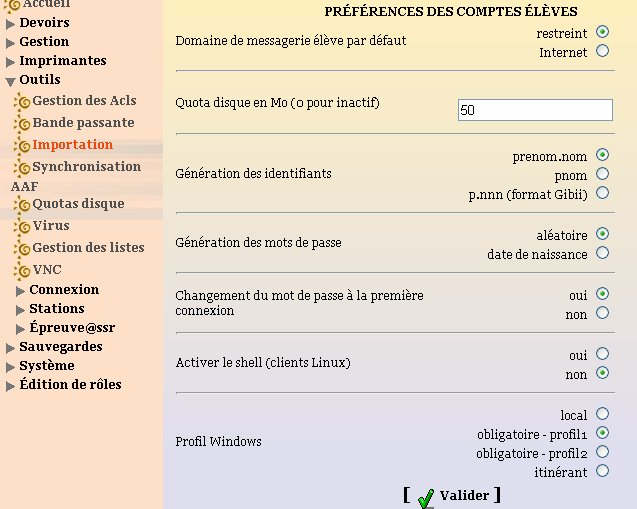
\includegraphics{scribe_html_10e3ad18.jpg}
\caption{Import des utilisateurs}
\end{figure}

il est aussi possible de passer par l'import d'un fichier plus
rudimentaire au format texte .csv dont voici une strucure type :

\begin{lstlisting}
"numero";"nom";"prenom";"sexe";"date";"classe";"niveau"
"0224ISWV7201";"DUPOND";"Norbert";"M";"07/12/1997";"3e1";"3"
"0544ETME3593";"MARTIN";"Maxence";"F";"04/09/1999";"4e1";"4"
"3887ELDEX3983";"DURAND";"Raoul";"M";"03/02/1999";"4e1";"4"
\end{lstlisting}
\subsection{Exercices sur la gestion des utilisateurs}

\begin{enumerate}[(1)]
\item
  Exercice : Créer les comptes à partir des fichiers sconet.

  \begin{itemize}
  \item
    Tester un ou deux des comptes créés.
  \item
    Dans l'EAD, accéder au compte d'un élève, lire les informations
    disponibles (en particulier le quota disque) et réinitialiser son
    mot de passe (en forçant sa modification à la 1ère connexion)
  \item
    Tester l'édition groupée pour réinitialisation tous les mots de
    passe des élèves.
  \end{itemize}
\item
  Exercice : Créez un nouvel élève, ayant les propriétés suivantes :
  \begin{itemize}
  \item
    Login : votreprenom.eleve (N ⇒ numéro donné par le formateur)
  \item
    prénom : le votre , nom = eleve , mot de passe = 1234
  \item
    Numéro interne de l'élève : 400N
  \item
    Quota disque = 50 Mo
  \item
    Date de naissance = date du jour
  \item
    Profil utilisateur = Obligatoire
  \item
    Classe : stage\_formation3
  \item
    Vérifier sa connexion et l'accès à ses partages dans le poste de
  \item
    Listez tous les élèves dont le login commence par un T
  \item
    Editez les propriétés d'un élève
  \item
    Editez les propriétés d'un professeur
  \end{itemize}
\item
  Exercice : Créez un nouveau professeur, ayant les propriétés suivantes
  : (Attention les caractères spécifiques tels que les accents sont
  interdits dans le nom de login)
  \begin{itemize}
  \item
    Login : votreprenom.prof
  \item
    prénom : le votre , nom = prof, mot de passe = 1234
  \item
    Quota disque = 100 Mo
  \item
    Profil utilisateur = Obligatoire
  \item
    Il n'est pas professeur principal, ni membre du groupe DomainAdmins
  \item
    Pas d'activation du Shell
  \end{itemize}
\item
  Exercice : L'utilisateur crée dans l'exercice précédent est professeur
  de mathématiques dans les classes 4e1 et 4e2
  \begin{itemize}
  \item
    Créez la matière Mathématiques
  \item
    Inscrivez-le dans sa matière, ses équipes pédagogiques et
    permettez-lui d'administrer la classe de 4e1
  \item
    Vérifier sa connexion et l'accès à ses partages dans le poste de
    travail.
  \item
    Se connecter à l'EAD en tant que professeur et vérifier son statut
    de professeur administrateur de la classe 4e1.
  \end{itemize}
\end{enumerate}
\subsection{Exercices sur la gestion des groupes}

\begin{enumerate}[(1)]
\setcounter{enumi}{4}
\item
  Exercice : Vérifier si le groupe «Documentation» existe. Dans la
  négative :
  \begin{itemize}
  \item
    créer un groupe de type Matières dont l'intitulé est
    «Documentation».
  \item
    Avec Partage et Modèle Données/Travail
  \item
    Pas de liste de diffusion
  \item
    Inclure les documentalistes dans le groupe ``Documentation'' (les
    créer si nécessaire et les associer à toutes les classes)
  \end{itemize}
\item
  Exercice : Créer un groupe «stage» ayant les propriétés suivantes :
  \begin{itemize}
  \item
    Type «groupe»
  \item
    Avec partage : Modèle Données/Travail
  \item
    Pas de liste de diffusion
  \item
    Membres : 3 élèves (penser à leur appartenance à une classe pour les
    affecter tous en une seule manipulation) et le professeur
    «votreprenom.prof».
  \item
    Lister les membres du groupe stage via l'EAD
  \item
    Vérifier la création du partage et les droits effectifs des
    utilisateurs
  \end{itemize}
\end{enumerate}
\section{4. ESU (Environnements Sécurisés des Utilisateurs)}

\subsection{Présentation}

ESU permet de gérer de façon la configuration de l'environnement de
l'utilisateur sur les stations Windows.Cette configuration est établie à
l'ouverture de la session, en fonction du nom de la machine et du groupe
d'utilisateurs auquel appartient l'utilisateur.

\begin{itemize}
\item
  ESU configure les environnements à partir de règles (des clés de la
  base de registre Windows) qui sont stockées dans le fichier XML
  \textless{}\textbackslash{}adresse\_serveur\textbackslash{}esu\textbackslash{}Console\textbackslash{}ListeRegles.xml\textgreater{}.
\item
  ESU permet de gérer le cragement des icônes du bureau et du menu
  démarrer. Ces icônes sont stockées dans le lecteur R: (icones\$). On
  trouve ici les dossiers correspondant aux groupes de machines définis
  dans ESU. Par exemple pour le groupe créé par défaut à l'installation
  de scribe,
\end{itemize}
\begin{figure}[htbp]
\centering
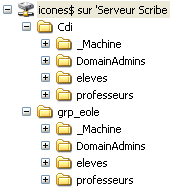
\includegraphics{scribe_html_6d99f570.png}
\caption{L'Arborescence du dossier icones\$}
\end{figure}

\begin{itemize}
\item
  les icônes placées dans seront visibles par tous les utilisateurs du
  groupe ;
\item
  les icônes placées dans ne seront visibles que par les professeurs du
  groupe ;
\item
  les éléments placés dans Démarrer s'afficheront dans le menu Démarrer
  des utilisateurs du groupe ;
\end{itemize}
Profils utilisateurs et ESU

Il est important de distinguer les profils utilisateurs (notion interne
à Windows) et ESU. Les profils utilisateurs sont appliqués en premier et
définissent un environnement de départ. La configuration ESU est
appliquée ensuite et modifie, ajoute ou supprime des paramètres de cet
environnement.

Par exemple, le menu démarrer est contenu dans le profil de
l'utilisateur mais si un chemin alternatif est défini dans ESU (Console
ESU : Windows -\textgreater{} Dossiers) alors, le menu démarrer utilisé
sera celui défini dans ESU, et non celui du profil.

Pour lancer la console, cliquez sur le raccourci présent dans le
répertoire personnel de l'utilisateur admin. Par défaut, seul
l'utilisateur admin a accès à la console.

\begin{figure}[htbp]
\centering
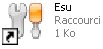
\includegraphics{scribe_html_5a76214.jpg}
\caption{Raccourci ESU}
\end{figure}

La console ESU sert à paramétrer les règles qui seront appliquées sur
les machines clientes lors de l'ouverture de session. Elles sont
réparties en deux groupes :

\begin{itemize}
\item
  les règles ``machines'' définissant le comportement global des
  machines, elles sont appliquées quelque soit l'utilisateur qui se
  connecte ;
\item
  les règles ``utilisateurs'' définissant l'environnement de
  l'utilisateur comme les restrictions, le paramétrage de l'explorateur
  et du fond d'écran, etc.
\item
  Chaque coche peut prendre 3 états :
\end{itemize}
\begin{figure}[htbp]
\centering

\includegraphics{scribe_html_4d04a591.png}
\caption{Les états dans ESU}
\end{figure}

\begin{enumerate}[1.]
\item
  cochée : Règle activée
\item
  décochée : Règle désactivée
\item
  grisée : Règle non prise en compte
\end{enumerate}
\begin{figure}[htbp]
\centering
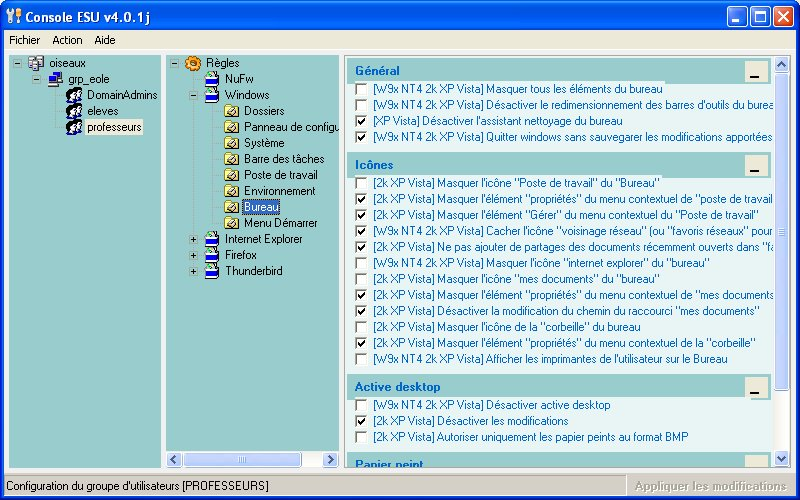
\includegraphics{scribe_html_3a7fb0ad.jpg}
\caption{image}
\end{figure}

\subsection{Règles de priorité dans l'application des règles ESU}

\end{document}
